%%%%%%%%%%%%%%%%%%%%%%%%%%%%%%%%%%%%%%%%%%%%%%%%%%%%%%%%%%%%%

\mainmatter%
\setcounter{page}{1}

\lectureseries[\course]{\course}

\auth[\lecAuth]{Lecturer: \lecAuth\\ Scribe: \scribe}
\date{January 26, 2010}

\setaddress%

% the following hack starts the lecture numbering at 1
\setcounter{lecture}{6}
\setcounter{chapter}{6}

\lecture{Stability \& Attractiveness}

\section{Basics}
\begin{definition}
The equilibrium point $x=0$ of $\dot{x}=f(x)$ is:
\begin{itemize}
\item \textit{stable} if $\forall \epsilon > 0~\exists~\delta=\delta(\epsilon)>0$ such that
\begin{align*}
|x(0)| < \delta \Rightarrow |x(t)| < \epsilon, \forall t\geq0,
\end{align*}
This means that the solution is bounded for any initial condition as in Figure~\ref{fig:07stableEqPoint}.
\item \textit{unstable} if the equilibrium point is not stable,
\item \textit{attractive} if there exists $\delta>0$ such that if $|x(0)|<\delta$ then
\begin{align*}
\lim_{t\to\infty}x(t) = 0,
\end{align*}
Attractiveness does not concern the rate of convergence or even stability of the system to the equilibrium point. Note that it is difficult to describe a real physical system that is attractive but not stable, however mathtematically it must be considered. See Figure~\ref{fig:07attractiveNotStable} for an example of a system that is attractive but not stable.
\item \textit{asymptotically stable} (a.s) if the equilibrium point is stable and attractive,
\item \textit{globally asymptotically stable} (g.a.s.) if the equilibrium point is a.s. $\forall x_0\in\mathbb{R}^n$.
\end{itemize}
\end{definition}

\begin{figure}[ht!]
\centering
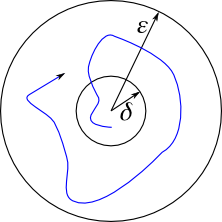
\includegraphics[width=.4\textwidth]{images/07stableEqPoint}
\caption{Stable equilibrium point.}
\label{fig:07stableEqPoint}
\end{figure}

\begin{definition}
Consider the system $\dot{x}=f(x)$ and a scalar valued $V(x)$. Then
\begin{align*}
\dot{V}(x) = \sum_{i=1}^n \frac{\partial V}{\partial x_i} f_i(x) = \frac{\partial V}{\partial x}f = \nabla V^T f = L_f V
\end{align*}
where $L$ is the Lie or directional derivative.
\end{definition}

\begin{figure}[ht!]
\centering
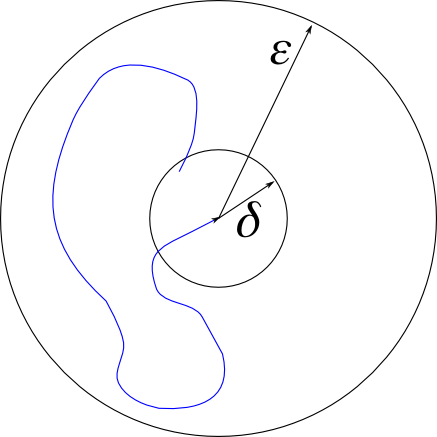
\includegraphics[width=.4\textwidth]{images/07attractiveNotStable}
\caption{Stable equilibrium point.}
\label{fig:07attractiveNotStable}
\end{figure}

\begin{theorem}{Lyapunov Stability}
Let $x=0$ be an equilibrium point of $\dot{x}=f(x)$ and let $V:D\to\mathbb{R}$, $D\in\mathbb{R}^n$.
\begin{enumerate}
\item If $V(0)=0$, $V(x)>0 \forall x \in D - \{0\}$ and $\dot{V}(x)\leq0 \forall x\in D$ then $x=0$ is stable.
\item If, in addition, $\dot{V}(x)<0 \forall x\in D-\{0\}$ then $x=0$ is a.s.
\end{enumerate}
\end{theorem}

The function $V$ can be thought of as the energy of the system.

\begin{example}
Let $\dot{x}=-\sin(x)$. The equilibria are at $x=k\pi$, $k\in\mathbb{Z}$ such as the equilibrium point at $x=0$. Let $V(x)=\tfrac{1}{2}x^2$, then $\dot{V}(x)=x\dot{x}=-x\sin(x)$. It can be seen that
\begin{itemize}
\item $\dot{V}(x) < 0 \forall x\in(-\pi,\pi)-\{0\}$,
\item the origin $x=0$ is a.s.
\end{itemize}
$\lozenge$
\end{example}

%%%%%%%%%%%%%%%%%%%%%%%%%%%%%%%%%%%%%%%%%%%%%%%%%%%%%%%%%%%%%
